\documentclass[a4paper, 11pt]{article}
\usepackage[top=3cm, bottom=3cm, left = 2cm, right = 2cm]{geometry}
\geometry{a4paper}
\usepackage[utf8]{inputenc}
\usepackage{textcomp}
\usepackage{graphicx}
\usepackage{amsmath,amssymb}
\usepackage{bm}
\usepackage[pdftex,bookmarks,colorlinks,breaklinks]{hyperref}
\hypersetup{linkcolor=black,citecolor=black,filecolor=black,urlcolor=black}
\usepackage{memhfixc}
\usepackage{pdfsync}
\usepackage{fancyhdr}
\pagestyle{fancy}

\title{Experimental Protocol}
\author{Kenneth Koski}
\date{CS224U}

\begin{document}
\maketitle

\section{Hypotheses}

The hypotheses examined in this paper are:

\begin{enumerate}
\item Few-shot learning with a transformer-based language model achieves top performance on the task of Named Entity Recognition (NER) on the Few-NERD dataset\cite{few-nerd}. This will be compared to a baseline of the NER modules available in the spaCy and nltk Python libraries, as well as an LSTM-based language model.

\item Few-shot learning with a transformer-based language model achieves top performance on the task of NER for Consumer Packaged Goods (CPG) brands on a small validation dataset manually curated from Reddit comments. This will be compared to a baseline of the NER modules available in the spaCy and nltk Python libraries, as well as an LSTM-based language model.

\item There is a high correlation between prompts that perform well on the Few-NERD dataset and prompts that perform well on the manually-curated dataset of Reddit comments.

\item Prompt engineering will make a considerable difference in how well a model performs on each dataset.
\end{enumerate}

See Figure~\ref{fig:example-prompts} for an example of some of the prompts that will be explored.

\begin{figure}
\centering
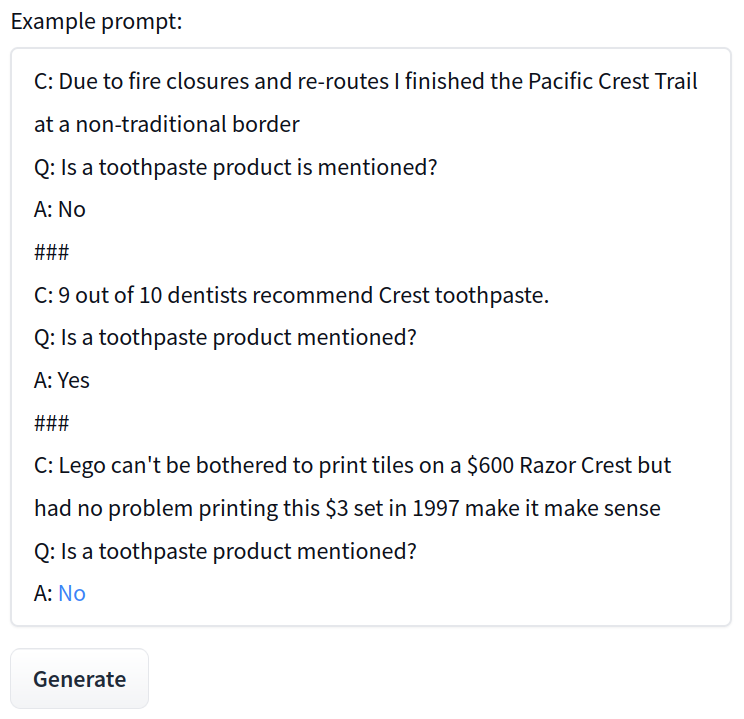
\includegraphics[scale=0.33]{example-prompts}
\caption{Example of prompts that will be explored}
\label{fig:example-prompts}
\end{figure}

\section{Datasets}

The main dataset used will be Few-NERD\cite{few-nerd}. It 8 coarse-grained types, 66 fine-grained types, 188,200 sentences, 491,711 entities and 4,601,223 tokens\cite{few-nerd}. Figure~\ref{fig:few-nerd-types} shows the available types in the dataset. This dataset was chosen primarily for two reasons, listed below.

\begin{figure}
\centering
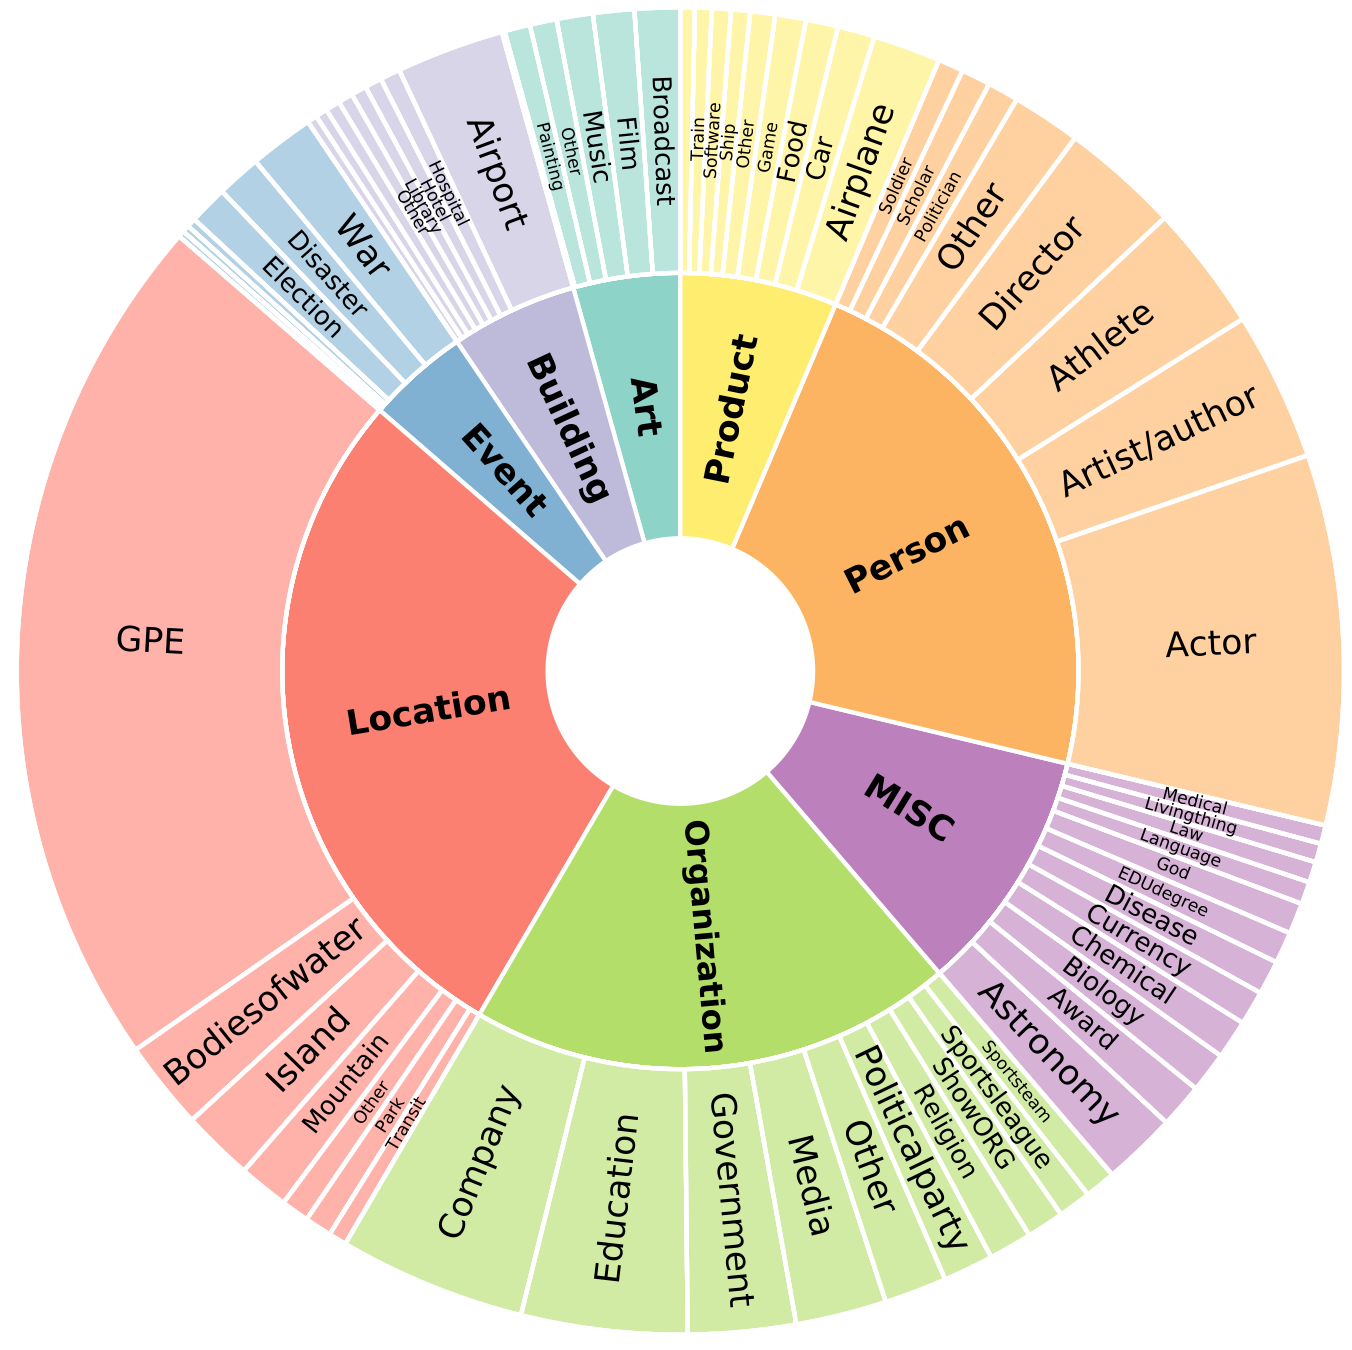
\includegraphics[scale=0.33]{few-nerd-types}
\caption{Visualization of coarse and fine-grained types available in Few-NERD}
\label{fig:few-nerd-types}
\end{figure}


\begin{enumerate}
\item It is a large-scale NER dataset, with approximately 15 times the number of tokens in the English-language portion of the CoNLL-2003 dataset\cite{conll-2003} (approximately 4.6 million vs 300,000), another dataset popular for the task of Named Entity Recognition.
\item Most NER datasets have labelled entities that are not relevant to the CPG space. The typical list is exemplified by the CoNLL-2003 dataset, which simply labels entities as \verb|LOC|, \verb|MISC|, \verb|ORG|, or \verb|PERS|. Although the \verb|ORG| label may potentially contain CPG-relevant companies and brands, the datasets tend to sample texts that do not contain many companies or brands. In contrast, the Few-NERD dataset contains very fine-grained labels, including the \verb|product-food| label, which contains some CPG-relevant brands. It is expected that this will help the hypothesis about high correlation between well-performing prompts on the two datasets hold.
\end{enumerate}


\section{Metrics}

Each model will be evaluated on F1-score for each dataset, as is common for the task of NER\cite{ner-eval}. Additionally, each model will be evaluated with the interpretable method proposed in \cite{ner-eval}.

\section{Models}

There will be 3 models used for this project, listed below.

\begin{enumerate}
\item The \verb|en_core_web_lg| model available in spaCy\cite{spacy}
\item The \verb|maxent_treebank_pos_tagger| model available in nltk\cite{nltk}
\item The \verb|BLOOM| model available on huggingface.co\cite{bloom}
\end{enumerate}

\section{General Reasoning}

The overall goal will be to explore how accurate a transformer-based large language model can perform at the task of Named Entity Recognition on both an existing NER dataset, as well as a dataset of Consumer Packaged Goods mentions manually-curated from Reddit comments.

The correlation between scores on the two datasets will be explored, with the assumption of high correlation. This is important for the goal of performing Named Entity Recognition for Consumer Packaged Goods brands, as there exists a paucity of datasets with relevant entities. Showing correlation here will allow for higher confidence that evaluating a model on a dataset with ample relevant entities can transfer into related-but-novel areas.

Prompt engineering will also be explored. This is expected to have a large impact on the performance of the transformer-based model. This is an exciting new area enabled by large language models, and has not yet been fully explored in the literature.

\section{Summary of Progress}

The Few-NERD dataset has been obtained and examined. The manually-curated CPG dataset is in the process of being created. An environment is being set up that has enough resources to run the \verb|BLOOM| model.

\bibliographystyle{abbrv}
\bibliography{experimental-protocol}
\end{document}
